\chapter{SCF Domain: Design and Implementation}
\label{chap:scf_domain}

\section{Introduction}
\label{sec:ch3_introduction}

Chapter II described the technical architecture that supports the platform. This chapter enters the business core of the system: the Supply Chain Finance domain model and its backend implementation. The aim is to explain how banking concepts such as counterparties, anchors, products, programs, invoices, fee catalogues, documents, and approval states become structured software objects.

The SCF service is not a collection of isolated controllers. It is organized around a domain where each entity participates in a larger financing chain. A counterparty may be onboarded and governed. A product definition describes a reusable financing template. A program turns that template into a concrete operating arrangement between an anchor, counterparties, limits, fees, cashflows, and disbursement rules. Documents and invoices then enrich that program with operational evidence.

\section{SCF Data Model: Entities and Relationships}
\label{sec:scf_data_model}

\subsection{BaseEntity: Shared Auditing and Governance Fields}
\label{subsec:base_entity}

All major SCF entities inherit from a shared \texttt{BaseEntity}. This base class provides the technical identity of each record, but its role goes further than an identifier. It carries fields for creation metadata, modification metadata, optimistic locking through a version field, approval status, pending action, maker user, checker user, and checker comments.

This design pushes governance into the entity model itself. Rather than treating approval as a temporary screen state, the platform stores it as part of the persistent record. That choice fits the banking context: a record is not only data; it also has an author, a lifecycle, a review status, and sometimes a rollback history.

\subsection{Core Business Entities}
\label{subsec:core_business_entities}

The core model revolves around counterparties, anchors, product definitions, program configurations, fee catalogues, cashflows, and documents. Figure~\ref{fig:ch3_core_data_model} summarizes the main structural relationships.

\begin{figure}[H]
    \centering
    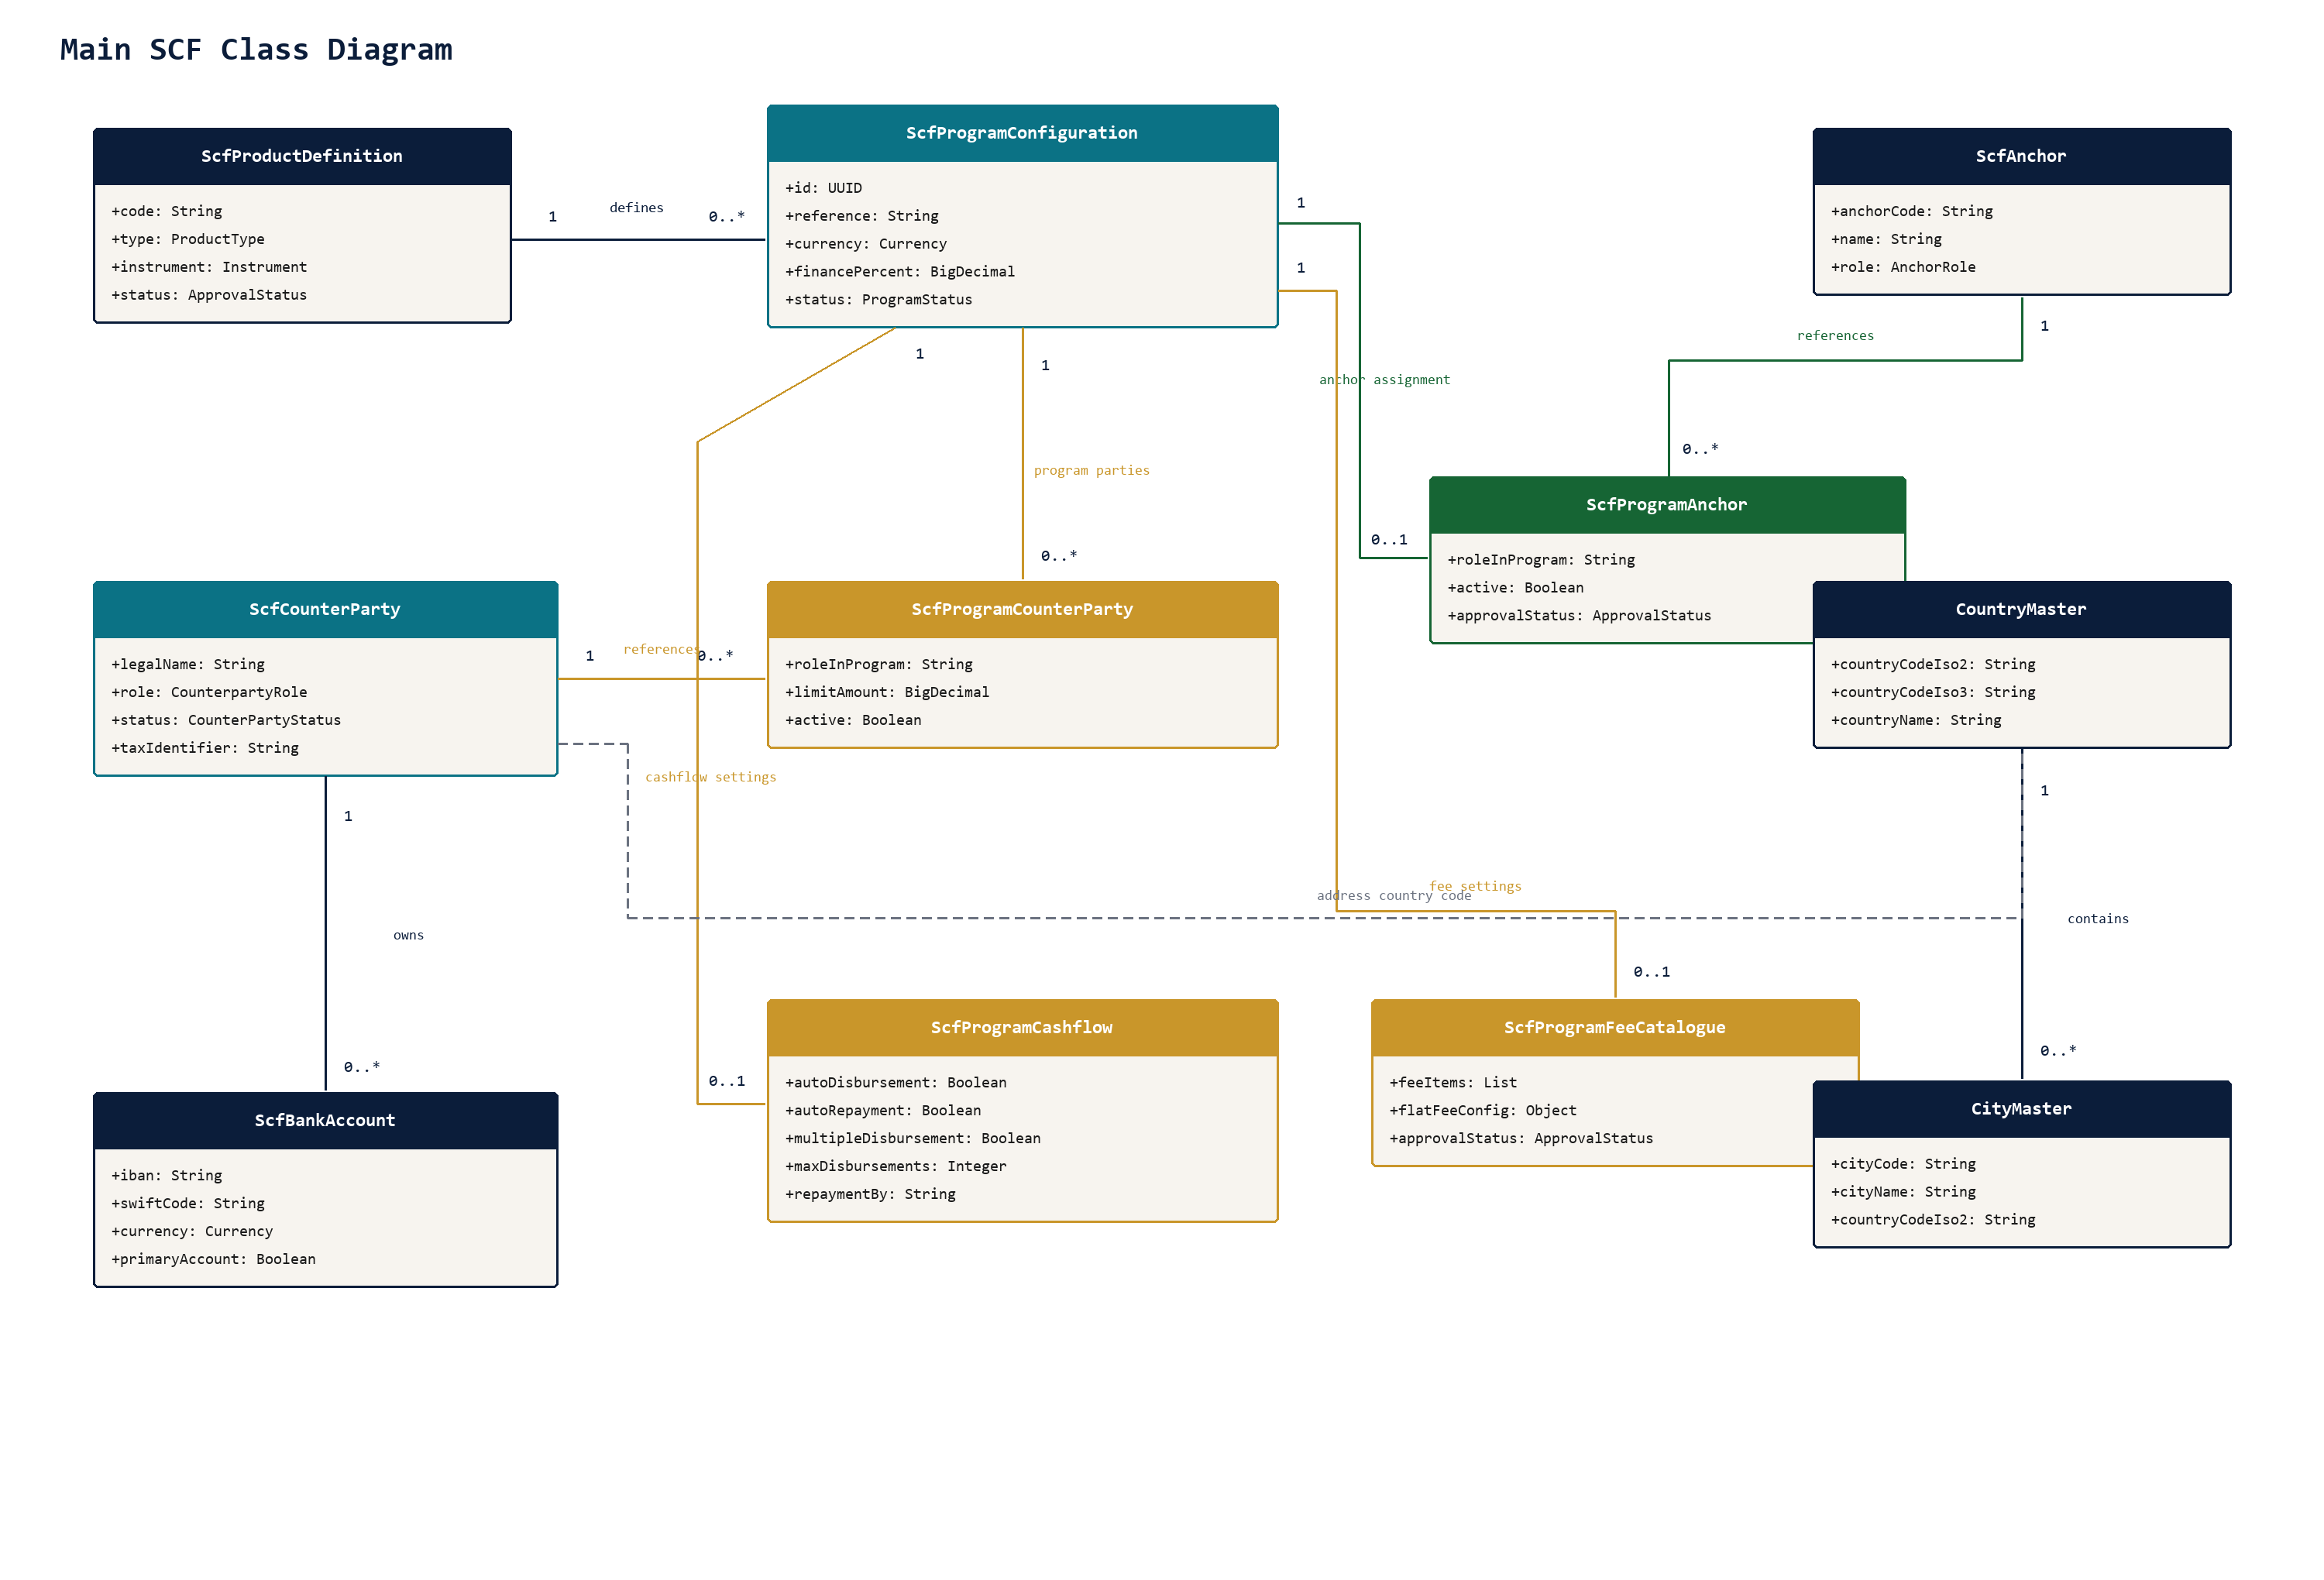
\includegraphics[width=\textwidth, keepaspectratio]{diagram_as_code/images/png/ch3_core_data_model.png}
    \caption{SCF core data model}
    \label{fig:ch3_core_data_model}
\end{figure}

\texttt{ScfCounterParty} represents a corporate, individual, or SME actor participating in trade finance. It stores company identity, legal identity, tax and registration information, contact information, address data, role, status, and rollback data. It is linked to \texttt{ScfBankAccount}, which stores banking details such as account number, IBAN, SWIFT code, currency, and primary-account flag. It is also linked to \texttt{ScfCounterPartyDocument}, which stores uploaded document metadata while the actual file bytes are kept in MinIO.

\texttt{ScfAnchor} represents the large corporate actor that structures a financing program. In many SCF products, the anchor's commercial strength is what gives the program its risk profile. The entity is linked to \texttt{ScfProgramAnchor}, a junction object that binds an anchor to a program with a program-specific role.

\texttt{ScfProductDefinition} is a reusable financing product template. It contains a product name, product code, product type, underlying instrument, description, and status. Its importance lies in the separation it creates: a product is generic, while a program is concrete.

\texttt{ScfProgramConfiguration} is the operational instance. It carries the program name, reference, dates, currency, finance limits, finance percentage, disbursement method, repayment method, grace period, penalty rate, discount rate, and lifecycle status. It is linked to anchors, counterparties, fee catalogues, and cashflows. This entity becomes the center of program execution.

\texttt{ScfProgramFeeCatalogue} contains fee configuration. Its design uses JSON-serialized structures: \texttt{feeItems}, converted through \texttt{FeeItemsJsonConverter}, and \texttt{flatFeeConfig}, converted through \texttt{FlatFeeConfigJsonConverter}. That design gives the program flexible fee structures without multiplying relational tables for every fee variation.

\texttt{ScfProgramCashflow} represents the disbursement and repayment configuration attached to a program. It is not an invoice table. It stores settings such as disbursement account, repayment account, automatic disbursement, automatic repayment, multiple-disbursement support, part-payment and pre-payment flags, maximum allowed disbursements, holiday treatment, repayment actor, penalty behavior, appropriation sequence, and insurance configuration.

\subsection{Business Enumerations}
\label{subsec:business_enumerations}

The entity model is supported by enumerations that constrain business values. Table~\ref{tab:ch3_enums} gives a compact reading of the most important ones.

\begin{table}[H]
    \centering
    \caption{Main SCF enumerations and their role}
    \label{tab:ch3_enums}
    \standardtable
    \begin{tabularx}{\textwidth}{B{0.30\textwidth} Y}
        \standardtablehead{\textbf{Enumeration} & \textbf{Business role}}
        \texttt{ProductType} & Defines supported product families such as reverse factoring, dynamic discounting, receivables finance, payables finance, and distributor finance. \\
        \texttt{UnderlyingInstrument} & Identifies the financial instrument behind the product, such as invoice, purchase order, bill of exchange, promissory note, or letter of credit. \\
        \texttt{CounterPartyStatus} & Tracks the operational status of a counterparty from draft and approval stages to active, suspended, closed, or rejected states. \\
        \texttt{ApprovalStatus} & Represents the governance state used by the maker/checker workflow. \\
        \texttt{PendingAction} & Records the intended operation waiting for checker review: create, update, delete, or none. \\
        \texttt{ProgramStatus} & Controls the lifecycle of a program configuration, including draft, pending approval, approved, active, suspended, closed, and rejected states. \\
    \end{tabularx}
    \standardtableend
\end{table}

Enumerations are more than code cleanliness. They protect the platform from ambiguous state values and make lifecycle transitions easier to reason about. In a financial system, that is not cosmetic. A free-text status is an invitation to inconsistency.

\section{Maker/Checker Governance Pattern}
\label{sec:maker_checker_pattern}

\subsection{Business Rationale}
\label{subsec:maker_checker_rationale}

The maker/checker mechanism applies the four-eyes principle to sensitive banking operations. A maker creates or modifies a record. A checker reviews it. The same user cannot play both roles on the same pending operation. This protects the platform against unilateral changes and creates an auditable division between input and approval.

The mechanism appears across several modules: counterparties, product definitions, program configurations, and reference data. It is therefore not a local trick implemented for one screen. It is a recurring governance pattern in the platform.

\subsection{Technical Implementation}
\label{subsec:maker_checker_technical}

Technically, the pattern is supported by shared entity fields and repository specifications. The \texttt{GovernanceSpecifications.excludeOwnPendingRecords(currentUser)} rule prevents a maker's own pending records from appearing in the checker's approval queue. Additional specifications filter by approval status and pending action.

Figure~\ref{fig:ch3_maker_checker_state} presents the lifecycle in simplified form.

\begin{figure}[H]
    \centering
    
\includegraphics[width=\textwidth, keepaspectratio]{images/ch3_maker_checker_state.png}
    \caption{Maker/checker governance lifecycle}
    \label{fig:ch3_maker_checker_state}
\end{figure}

On creation, a record starts in draft form. When the maker submits it, the record becomes pending approval and carries the corresponding pending action. The checker can approve the operation, which validates the change, or reject it with comments. For updates, rejection can trigger a rollback through \texttt{OriginalDataRestorer}.

\subsection{OriginalDataRestorer}
\label{subsec:original_data_restorer}

\texttt{OriginalDataRestorer} serializes the previous entity state into the \texttt{originalData} field before modification. If the checker rejects the change, the stored snapshot is deserialized and applied back to the entity. This gives rejection a material effect. The record does not simply receive a rejected label; it can return to its previous approved state.

The mechanism is especially useful for update and delete requests. A pending update should not destroy the last approved business version until a checker accepts it. By preserving the original data, the system keeps both intent and recoverability.

\section{Counterparty Module}
\label{sec:counterparty_module}

\subsection{Business Purpose}
\label{subsec:counterparty_business_purpose}

The counterparty module manages actors that participate in financing programs. A counterparty can be a supplier, buyer, SME, or corporate actor. It must be identified, described, linked to bank accounts, enriched with documents, and governed through approval.

This module is one of the first operational gates in the SCF value chain. A program cannot reliably finance an invoice if the counterparties behind that invoice are poorly identified. The counterparty record therefore becomes a master object for later program configuration and transaction processing.

\subsection{Onboarding Workflow}
\label{subsec:counterparty_onboarding}

The controller package contains \texttt{CounterPartyController} and \texttt{CounterPartyDocumentController}. The main controller exposes operations for paginated listing, single fetch, creation, update, deletion, submission, approval, rejection, bulk creation, and CSV export. The document controller manages upload, listing, viewing through presigned URLs, direct download, and deletion.

The onboarding workflow follows a disciplined sequence. A bank maker creates a draft counterparty with company data, tax or registration identifiers, contact information, address fields, and bank accounts. The maker submits the record. A bank checker, different from the maker, reviews the pending operation and approves or rejects it.

\subsection{Document Management for Counterparties}
\label{subsec:counterparty_documents}

Counterparty documents are uploaded through multipart requests. The gateway can scan the file through ClamAV before the request reaches the SCF service. The service then stores file bytes through the object storage port and saves metadata in \texttt{ScfCounterPartyDocument}. Viewing can use a presigned URL, while download can stream the file directly.

The design keeps business metadata separate from binary storage. PostgreSQL stores the document record; MinIO stores the actual object. This separation avoids loading heavy files into relational rows and keeps retrieval logic explicit.

\section{Product Definition Module}
\label{sec:product_definition_module}

\subsection{Product Versus Program}
\label{subsec:product_vs_program}

The product definition module manages reusable templates. A product definition states what type of financing product is available and what underlying instrument supports it. A program configuration, by contrast, binds a product idea to concrete parties, limits, dates, fees, and disbursement rules.

This distinction avoids duplication. The bank can define a product category once, then configure multiple programs from it. The implementation reflects this separation through \texttt{ScfProductDefinitionServiceImpl}, the product mapper, the product repository, and product-specific exceptions such as duplicate code or unsupported ordering.

\subsection{Product Definition Lifecycle}
\label{subsec:product_definition_lifecycle}

Product definitions follow a CRUD and maker/checker lifecycle. The platform validates uniqueness of the product code and manages status transitions through governance fields. In business terms, this prevents uncontrolled product activation. In technical terms, it keeps product metadata consistent before programs depend on it.

\section{Program Configuration Module}
\label{sec:program_configuration_module}

\subsection{What a Program Represents}
\label{subsec:program_represents}

A program is the executable configuration of a financing relationship. It combines the product family, the anchor, counterparties, finance limits, currency, dates, fee structure, disbursement method, repayment method, and lifecycle status. It is the point where generic SCF theory becomes a concrete operational arrangement.

The OpenAPI file confirms a step-based program configuration style: general information, cashflow or disbursement-repayment settings, fee catalogue, submission, and copy. The implementation context also identifies \texttt{ProgramConfigurationController}, \texttt{CashflowUpdateController}, \texttt{FeeCatalogueUpdateController}, \texttt{ProgramConfigurationService}, \texttt{CashflowUpdateService}, \texttt{FeeCatalogueUpdateService}, and \texttt{ProgramSnapshotService}.

\subsection{Program Creation Flow}
\label{subsec:program_creation_flow}

Figure~\ref{fig:ch3_program_configuration_flow} summarizes the program configuration flow as a sequence of functional steps.

\begin{figure}[H]
    \centering
    
\includegraphics[width=\textwidth, keepaspectratio]{images/ch3_program_configuration_flow.png}
    \caption{Program configuration functional flow}
    \label{fig:ch3_program_configuration_flow}
\end{figure}

The first step gathers general data: program name, reference, dates, currency, product type, finance limits, anchor assignment, and counterparty assignment. The fee step configures fee items and flat fee settings. The cashflow step configures disbursement and repayment behavior. Once the draft is complete, the program can be submitted into the approval lifecycle.

\subsection{Fee Catalogue Structure}
\label{subsec:fee_catalogue_structure}

The fee catalogue is one of the more flexible parts of the model. Each \texttt{ProgramFeeItem} can include fee type, calculation basis, rate, flat amount, currency, and frequency. The \texttt{FlatFeeConfig} stores flat-fee-level settings. Both are serialized as JSON through dedicated converters.

This approach accepts the variability of banking fees without forcing every possible fee structure into rigid columns. The trade-off is that validation must be handled carefully in the service layer, because JSON flexibility can otherwise hide malformed business data.

\subsection{Program Copy Feature}
\label{subsec:program_copy}

\texttt{ProgramSnapshotService} supports copying an existing program. It duplicates reusable configuration and its sub-entities, including anchors, counterparties, fee catalogues, and the program cashflow settings. The copied program starts in draft status.

This behavior is coherent because the backend cashflow object is a configuration object, not transactional invoice history. The feature therefore copies reusable program settings while keeping operational records, such as uploaded invoices and financing transactions, outside the program-copy operation.

\section{Program Cashflow Configuration and Invoice Upload}
\label{sec:invoice_cashflow}

\subsection{Disbursement and Repayment Cashflow Configuration}
\label{subsec:cashflow_validation}

In the backend implementation, cashflow management refers to the program's disbursement and repayment setup. The \texttt{CashflowUpdateController} accepts a \texttt{ProgramCashflowRequest} for a target program and delegates the update to \texttt{CashflowUpdateService}. The service loads the program configuration, creates the associated \texttt{ScfProgramCashflow} if it does not already exist, validates the submitted policy fields, applies the mapper, and persists the result.

\begin{algorithm}[H]
    \DontPrintSemicolon
    \Data{Program identifier and submitted disbursement/repayment settings}
    \Result{Updated program cashflow configuration}
    \BlankLine
    Load the target program configuration\;
    Validate insurance policy fields and related configuration values\;
    \If{no cashflow object exists for the program}{
        Create a new \texttt{ScfProgramCashflow} linked to the program\;
    }
    Apply the submitted settings through the mapper\;
    Save the updated cashflow configuration\;
    Return the program cashflow response\;
    \caption{Program cashflow update routine}
    \label{alg:cashflow_update}
\end{algorithm}

Invoice upload remains a separate operational flow. In the current sprint context, invoice upload and finance-disbursement preview screens still use transitional frontend services while the platform migrates these flows toward native Spring Boot endpoints. This separation avoids confusing two different concepts: program cashflow configuration defines how disbursement and repayment should behave, while uploaded invoices represent operational evidence that can later become eligible for financing.

\section{Transaction Inquiry Module}
\label{sec:transaction_inquiry_module}

The transaction inquiry module provides filtering and consultation of operational records. On the frontend side, \texttt{SCFTransactionInquiry} displays filters and a transaction table. Row actions can open invoice or finance disbursement views. On the backend side, this module depends on the consistency of the domain model: transactions are meaningful only if programs, counterparties, invoices, and disbursement records have been structured properly upstream.

The module is therefore a reading surface over the work performed by the other modules. It gives bank officers, anchors, or counterparties a controlled way to inspect the state of financing operations.

\section{Conclusion}
\label{sec:ch3_conclusion}

This chapter analyzed the SCF domain model and the backend modules that implement it. The data model is built around counterparties, anchors, product definitions, program configurations, fee catalogues, cashflows, and documents. Governance is embedded through shared entity fields, approval statuses, pending actions, repository specifications, and rollback snapshots. The program module stands at the center of the system because it turns reusable products into concrete financing arrangements.

The next chapter shifts from backend domain implementation to frontend implementation. It studies how these business concepts are exposed through React components, role-based navigation, forms, wizards, service calls, and user-facing flows.
